\section{Presa Dati}
\subsection{Efficienza dei rivelatori e distanze apparato sperimentale}\label{eff}
Per trovare l'efficienza totale dei rivelatori si è utilizzato lo schema in Figura \ref{immagine efficienza rivelatori}.
\begin{figure}[h]
    \centering
    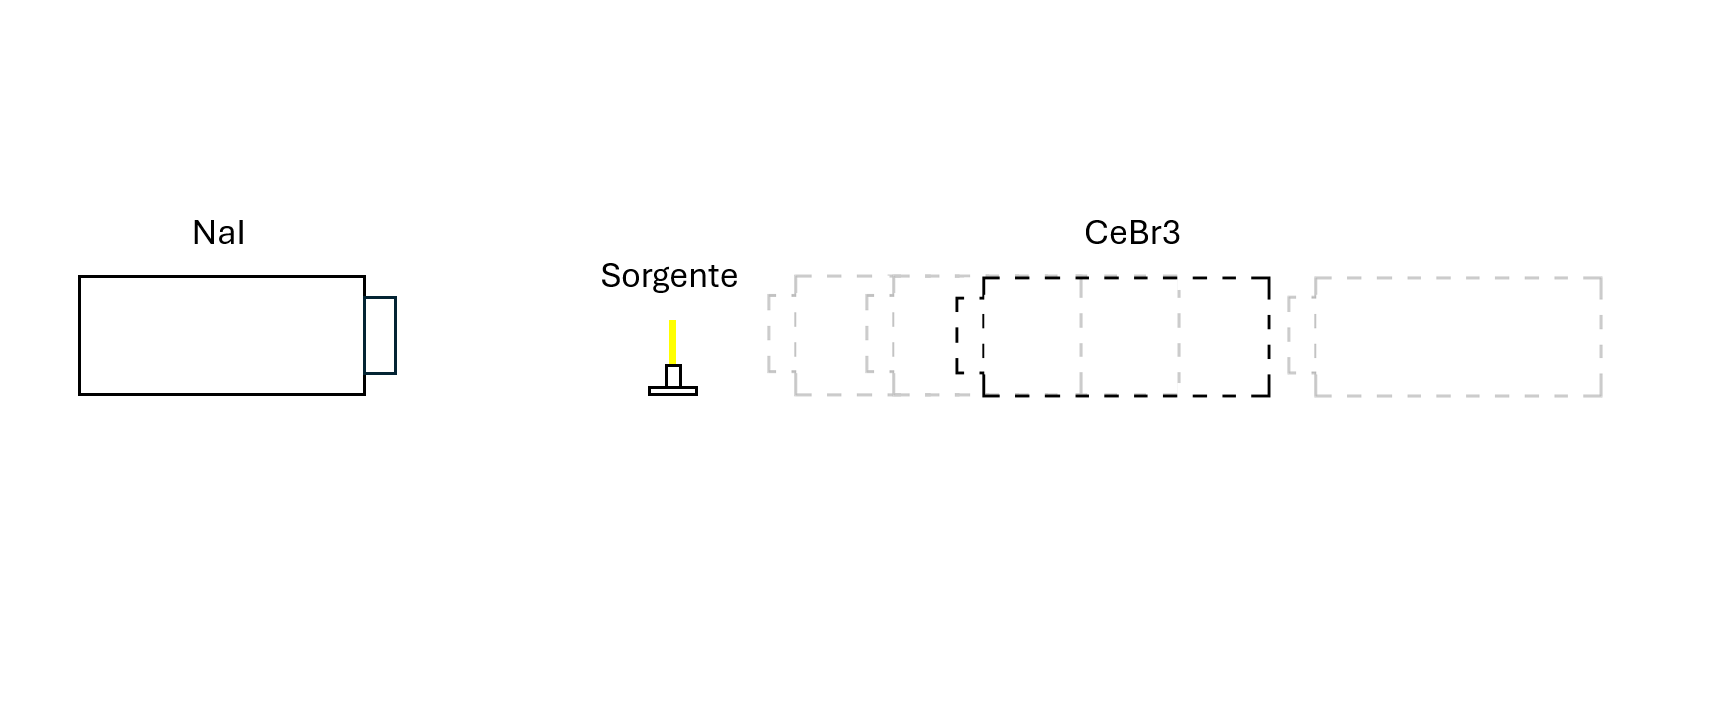
\includegraphics[width=0.85\textwidth]{Presa dati/Plateau efficienza.png}
    \caption{Raffigurazione della disposizione dei rivelatori per calcolare l'efficienza}
    \label{immagine efficienza rivelatori}
\end{figure}

Per calcolare l'efficienza totale dei rivelatori si è calcolato il rapporto tra i conteggi del rivelatore al $\ch{CeBr_{3}}$ ottenuti con l'aiuto del programma MAESTRO e i conteggi del gate, ovvero quelli rivelatore al $\ch{NaI}$ ottenuti mediante un contatore NIM; in formula:
\begin{equation}
    \text{Efficienza}_\text{tot}=\frac{\text{Conteggi}_{\ch{CeBr_3}}}{\text{Conteggi}_{\ch{NaI}}}
\end{equation}
Come si può notare dalla figura soprastante i conteggi sono stati ottenuti mantenendo fissa a $15 \,\unit{cm}$ la distanza tra la sorgente di $\ch{^{22}Na}$ e il rivelatore gate e spostando manualmente il rivelatore al $\ch{CeBr_3}$ a distanze fissate.
I valori sono stati presi in un intervallo di tempo di 60 secondi per ogni misura e sono riportati in tabella \ref{tabella efficienza}.
\begin{table}[H]
    \centering
    \begin{tabular}{|c|c|c|c|}
    \hline
       dist. $\ch{CeBr_{3}}$-sorgente [$\unit{cm}$] & cont. $\ch{CeBr_{3}}$ & cont. gate ($\ch{NAI}$) & Efficienza (\%) \\
    \hline
    \hline
    $7$ & $11095$ & $17746$ & $62.52$ \\
    \hline
    $14$ & $11007$ & $18062$ & $60.94$ \\
    \hline
    $15$ & $10897$ & $17770$ & $61.32$ \\
    \hline
    $16$ & $10817$ & $18154$ & $59.58$ \\
    \hline
    $17$ & $10582$ & $18120$ & $58.40$ \\
    \hline
    $18$ & $9553$ & $17834$ & $59.34$ \\
    \hline
    $20$ & $9231$ & $18041$ & $51.17$ \\
    \hline
    $30$ & $4667$ & $17982$ & $25.95$ \\
    \hline
    \end{tabular}
    \caption{Sono presentati i vari valori utilizati per il calcolo dell'efficienza dei rivelatori.}
    \label{tabella efficienza}
\end{table}
Nel grafico sottostante si può notare come si formi il cosiddetto \textit{plateau} intorno a $15 \,\unit{cm}$.
\begin{figure}[H]
  \centering
  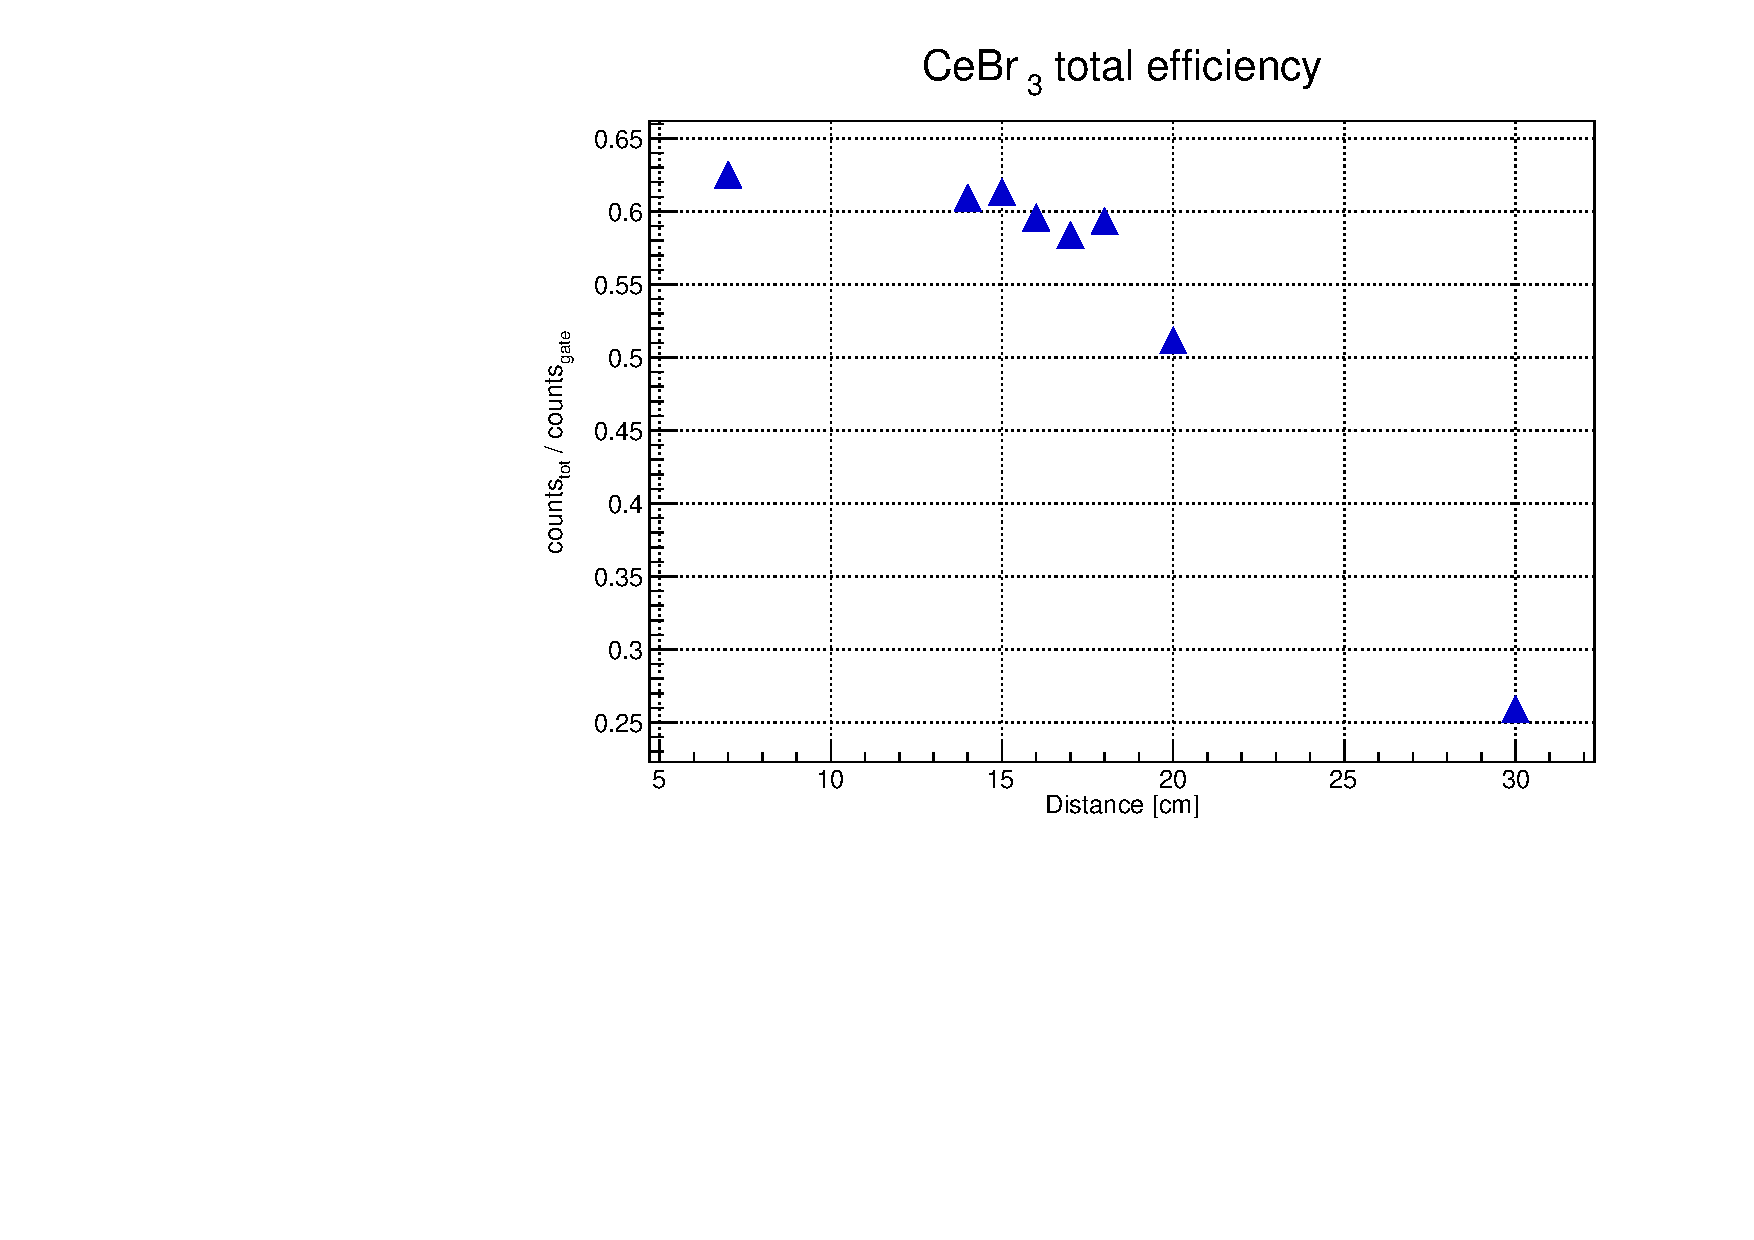
\includegraphics[scale=0.6]{Analisi Dati/tot_eff.pdf} 
  \caption{Plateau dell'efficienza del rivelatore}
  \label{fig:eff_tot}
\end{figure}
Date le considerazioni della sezione precedente si è deciso di fissare la distanza tra sorgente e $\ch{CeBr_{3}}$ a $15 \,\unit{cm}$ per vari motivi: prima di tutto perché è dove si trova il plateu; in secondo luogo perché mettendolo troppo vicino si osserverebbero effetti di \textit{pile-up} e il rivelatore vedrebbe anche particelle deviate a grande angolo pur non essendo angolato.
Inolre questo è un valore comodo per le altre lunghezze presenti nell'apparato sperimentale: infatti si sono calcolate le distanze tra sorgente e $\ch{NaI}$ e tra bersaglio e $\ch{CeBr_{3}}$ in modo tale da aver lo stesso angolo solido che si ha tra la sorgente e il bersaglio posto a $15\,\unit{cm}$. Per il calcolo degli angoli solidi tra la sorgente e bersaglio e tra sorgente e $\ch{NaI}$ la sorgente è stata considerata puntiforme, mentre per l'angolo solido tra bersaglio e rivelatore $\ch{CeBr_{3}}$ è stato considerato puntiforme e centrato il punto di interazione del fotone con il bersaglio di $\ch{Al}$. I valori delle distanze ottenuti sono riportati nella tabella sottostante.
\begin{table}[H]
    \centering
    \begin{tabular}{|c|c|}
    \hline
    $\text{Distanza} \quad \ch{NaI}-\text{sorgente}$ & $13.5\, \unit{cm}$ \\
    \hline
    $\text{Distanza} \quad \text{sorgente}-\text{bersaglio} (\text{fissata})$ & $15 \,\unit{cm}$ \\
    \hline
    $\text{Distanza} \quad \text{bersaglio}-\ch{CeBr_{3}}$ & $14.4\,\unit{cm}$ \\
    \hline
    \end{tabular}
    \caption{Sono presentati i vari valori delle distanze dell'apparato sperimentale.}
    \label{tabella efficienza}
\end{table}
%sarebbe utile indicare nella tabella come abbiamo chiamato le varie distanze. Quindi con l o d 
Per l'efficienza fotoelettrica sono state utilizzate le stesse misure dell'efficienza totale con la differenza che attraverso l'analisi dati si sono selezionati solo i conteggi del picco fotoelettrico. I valori ottenuti sono riportati nel grafico sottostante.
\begin{figure}[H]
  \centering
  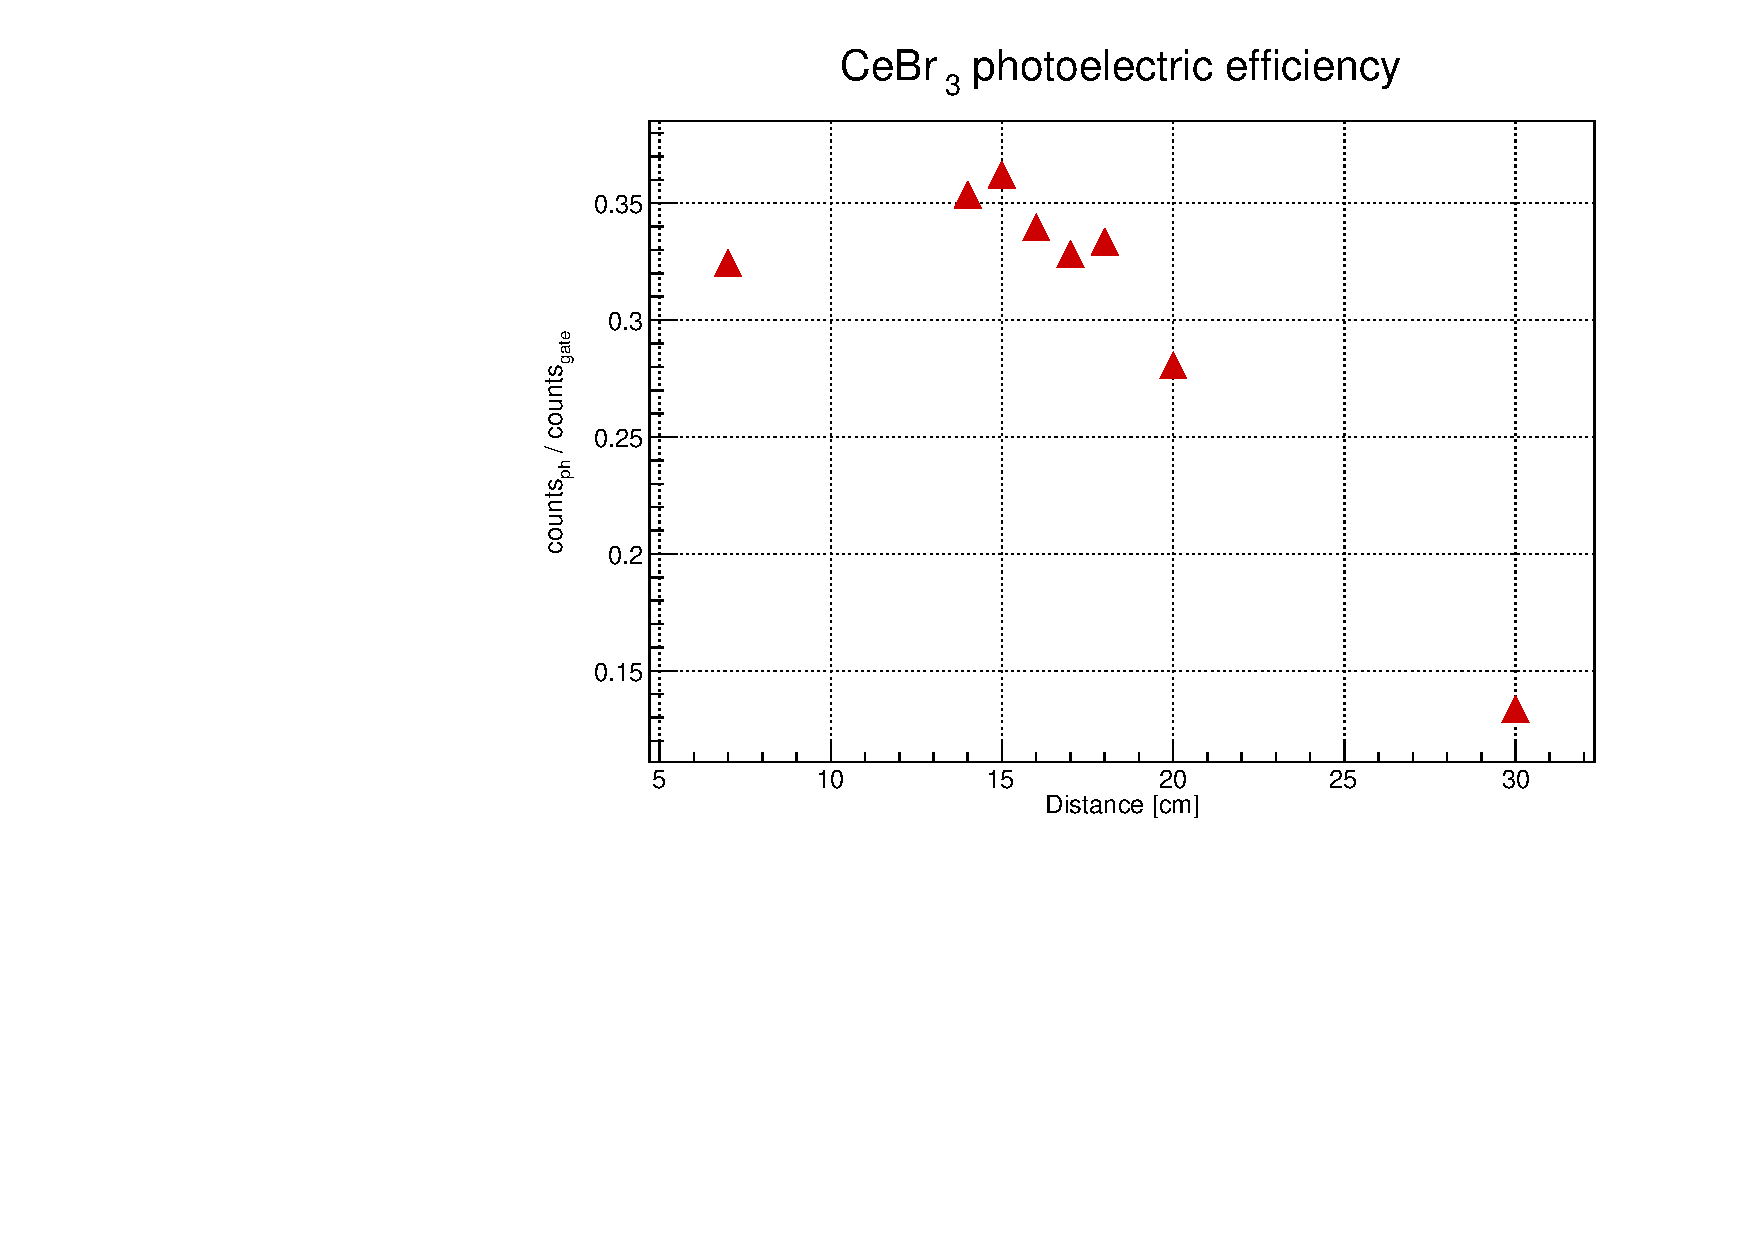
\includegraphics[scale=0.6]{Analisi Dati/ph_eff.pdf} 
  \caption{Plateau dell'efficienza fotoelettrica del rivelatore}
  \label{fig:eff_ph}
\end{figure}
\subsection{Misure della sezione d'urto}
Per quel che riguarda le misure a vari angoli sono stati stabiliti i valori di $30^\circ$, $45^\circ$, $60^\circ$ e $90^\circ$. Per uniformità tra le varie misure si è deciso di segnare sulla carta millimetrata il centro del bersaglio; questo è stato punto di riferimento dal quale sono state prese le misure di distanza bersaglio-rivelatore A nelle misure a vari angoli. Come visibile in fig. \ref{fig:schema_misura_distanze} il punto marcato ha consentito di misurare la distanza $l$ %non si capisce bene che cosa rappresenta la distanza l
a partire dal centro del bersaglio; inoltre risultava comodo per misurare accuratamente la disposizione angolare tramite il goniometro.

\begin{figure}[H]
    \centering
    \includegraphics[scale=0.15]{Errori/schema_distanze.png}
    \caption{Schematizzazione delle misure delle distanze. In rosso: distanza sorgente - bersaglio. In verde: distanza bersaglio - rivelatore A.}
    \label{fig:schema_misura_distanze}
\end{figure}
Le prese dati sono durate svariate ore a seconda del valore dell'angolo che veniva misurato e i valori di sezione d'urto, calolati con la formula \ref{eq sezione d'urto conteggi}, sono riportati nella Tabella \ref{tabella sezione d'urto}.
Inizialmente erano stati presi i dati anche per misure di $75^\circ$ e $120^\circ$, ma dopo qualche giorno di presa dati ci siamo subito accorti che i conteggi rilevati dal modulo \textit{NIM} subivano un reset dopo un certo tempo trascorso, probabilmente legato alla capacitá di memoria disponibile nel modulo stesso. A causa di ció le uniche misure di conteggi utilizzabili sono risultate quelle a $30^\circ$, $45^\circ$, $60^\circ$ e $90^\circ$ in quanto erano state effettuate in un tempo tale da non subire il reset del counter.
\begin{table}[H]
    \centering
    \begin{tabular}{|c|c|c|}
    \hline
       Angolo & $d\sigma/d\theta$ [$\num{e-26}\unit{cm^{2}/sr}$] & Errore sezione d'urto [$\num{e-27}\unit{cm^{2}/sr}$] \\
    \hline
    \hline
    $30^\circ$ & $3.92$ & $5.58$ \\
    \hline
    $45^\circ$ & $3.15$ & $4.48$ \\
    \hline
    $60^\circ$ & $2.50$ & $3.56$ \\
    \hline
    $90^\circ$ & $1.92$ & $2.73$ \\
    \hline
    \end{tabular}
    \caption{Sono presentati i vari valori ottenuti per la sezione d'urto.}
    \label{tabella sezione d'urto}
\end{table}
Gli errori associati alle misure e l'analisi dati sono esposti nella sezione \ref{sezione d'urto e montecarlo}.